% Options for packages loaded elsewhere
\PassOptionsToPackage{unicode}{hyperref}
\PassOptionsToPackage{hyphens}{url}
%
\documentclass[
  11pt,
]{article}
\usepackage{lmodern}
\usepackage{amssymb,amsmath}
\usepackage{ifxetex,ifluatex}
\ifnum 0\ifxetex 1\fi\ifluatex 1\fi=0 % if pdftex
  \usepackage[T1]{fontenc}
  \usepackage[utf8]{inputenc}
  \usepackage{textcomp} % provide euro and other symbols
\else % if luatex or xetex
  \usepackage{unicode-math}
  \defaultfontfeatures{Scale=MatchLowercase}
  \defaultfontfeatures[\rmfamily]{Ligatures=TeX,Scale=1}
  \setmainfont[]{Times New Roman}
\fi
% Use upquote if available, for straight quotes in verbatim environments
\IfFileExists{upquote.sty}{\usepackage{upquote}}{}
\IfFileExists{microtype.sty}{% use microtype if available
  \usepackage[]{microtype}
  \UseMicrotypeSet[protrusion]{basicmath} % disable protrusion for tt fonts
}{}
\makeatletter
\@ifundefined{KOMAClassName}{% if non-KOMA class
  \IfFileExists{parskip.sty}{%
    \usepackage{parskip}
  }{% else
    \setlength{\parindent}{0pt}
    \setlength{\parskip}{6pt plus 2pt minus 1pt}}
}{% if KOMA class
  \KOMAoptions{parskip=half}}
\makeatother
\usepackage{xcolor}
\IfFileExists{xurl.sty}{\usepackage{xurl}}{} % add URL line breaks if available
\IfFileExists{bookmark.sty}{\usepackage{bookmark}}{\usepackage{hyperref}}
\hypersetup{
  pdftitle={Online supporting information for Studying predator foraging mode and hunting success at the individual level with an online videogame},
  hidelinks,
  pdfcreator={LaTeX via pandoc}}
\urlstyle{same} % disable monospaced font for URLs
\usepackage[margin=1in]{geometry}
\usepackage{graphicx}
\makeatletter
\def\maxwidth{\ifdim\Gin@nat@width>\linewidth\linewidth\else\Gin@nat@width\fi}
\def\maxheight{\ifdim\Gin@nat@height>\textheight\textheight\else\Gin@nat@height\fi}
\makeatother
% Scale images if necessary, so that they will not overflow the page
% margins by default, and it is still possible to overwrite the defaults
% using explicit options in \includegraphics[width, height, ...]{}
\setkeys{Gin}{width=\maxwidth,height=\maxheight,keepaspectratio}
% Set default figure placement to htbp
\makeatletter
\def\fps@figure{htbp}
\makeatother
\setlength{\emergencystretch}{3em} % prevent overfull lines
\providecommand{\tightlist}{%
  \setlength{\itemsep}{0pt}\setlength{\parskip}{0pt}}
\setcounter{secnumdepth}{-\maxdimen} % remove section numbering
\usepackage{float}
\let\origfigure\figure
\let\endorigfigure\endfigure
\renewenvironment{figure}[1][2] {
    \expandafter\origfigure\expandafter[H]
} {
    \endorigfigure
}
\usepackage{lineno}\linenumbers
\usepackage{amsmath}
\usepackage{setspace}\doublespacing
\usepackage[labelfont=bf]{caption}
\captionsetup{singlelinecheck = false}
\captionsetup[figure]{name = Figure S}
\usepackage{sectsty}\allsectionsfont{\centering}
\usepackage{graphicx}
\newlength{\cslhangindent}
\setlength{\cslhangindent}{1.5em}
\newenvironment{cslreferences}%
  {}%
  {\par}

\title{Online supporting information for\\
Studying predator foraging mode and hunting success at the individual
level with an online videogame}
\author{}
\date{\vspace{-2.5em}}

\begin{document}
\maketitle

\newpage

\hypertarget{supporting-information-materials-and-methods}{%
\subsubsection*{Supporting Information: Materials and
methods}\label{supporting-information-materials-and-methods}}
\addcontentsline{toc}{subsubsection}{Supporting Information: Materials
and methods}

\begin{center}
\emph{Principal component analysis}
\end{center}

We computed a principal component analysis (PCA) using the packages
`FactoMineR' version 2.4 (Lê et al. 2008) and `factoextra' version 1.0.7
(Kassambara and Mundt 2020 Apr 1) in the R software version 4.0.4 (R
Core Team, 2021), under a Windows 10 Home computer OS (version 21H2, OS
build 19044.1466). The `PCA()' function in `FactoMineR' uses singular
value decomposition. Before running the PCA, we divided each variable
(except travel speed) by the match duration (seconds) to account for
differences in game lenght among matches. We applied a square-root
transformation to all the varialbes. They were then standardized to mean
and unit variance (Z scores) before running the PCA. We then ranked the
variables based on their relative contribution (in \%) to a given
principal component axis. To do so, for each variable, we used the ratio
between their cos2 multiplied by 100 and the cos2 of the principal
component.

\begin{center}
\emph{Parametrization of the Bayesian multivariate mixed-model}
\end{center}

We used a half-normal prior with mean of 0 and standard deviation of 1
for all the variance parameters, and applied a weakly informative LKJ
prior with a shape parameter (\(n\)) set to 2 for the random effects
variance-covariance matrices. We applied a Gaussian prior with mean of 0
and standard deviation of 2 for the fixed effects (i.e.~prey travel
speed \(x_1\) and rate of space covered \(x_2\)) of all the submodels
(i.e.~for each response variable). We set the model to run 4 chains with
2500 iterations where samples were drawn at every 8 intervals
(thinning), and to use the first 500 iterations as warmups. We visually
inspected the trace plots, effective sample sizes, and residuals to
assess convergence and stability. We also evaluated the model's
prediction accuracy using posterior predictive checks. We computed a
variance-covariance matrix (\(\Omega_{k}\)) for each random effect
(\(k\)). We extracted the among-environment, among-individual, and
within-individual variance components and behavioral correlations using
the function `as\_draws\_df()' in the `brms' package (for details,
consult the code files on the GitHub repository :
\url{https://github.com/quantitative-ecologist/predator-foraging-mode-videogames}).
We could thus compute the mean of the variance and correlation sample
values, and the HDP intervals to obtain their 95\% credible intervals.
The variance-covariance matrixes were parametrized as :

\[
\begin{bmatrix}
en_{0y1,g} \\ 
en_{0y2,g} \\ 
en_{0y3,g} \\
en_{0y4,g}
\end{bmatrix}
= MVN(0, \Omega_{en}) : \text{where } \Omega_{en} = 
\begin{bmatrix}
V_{en_{0y1}} & & & \\
Cov_{en_{0y1}en_{0y2}} & V_{en_{0y2}} & & \\ 
Cov_{en_{0y1}en_{0y3}} & Cov_{en_{0y1}en_{0y4}} & V_{en_{0y3}} & \\
Cov_{en_{0y2}en_{0y3}} & Cov_{en_{0y2}en_{0y4}} & Cov_{en_{0y3}en_{0y4}} & V_{en_{0y4}}
\end{bmatrix}
\tag{S1}
\]

\[
\begin{bmatrix}
av_{0y1,h} \\ 
av_{0y2,h} \\ 
av_{0y3,h} \\
av_{0y4,h}
\end{bmatrix}
= MVN(0, \Omega_{av}) : \text{where } \Omega_{av} = 
\begin{bmatrix}
V_{av_{0y1}} & & & \\
Cov_{av_{0y1}av_{0y2}} & V_{av_{0y2}} & &\\ 
Cov_{av_{0y1}av_{0y3}} & Cov_{av_{0y1}av_{0y4}} & V_{av_{0y3}} & \\
Cov_{av_{0y2}av_{0y3}} & Cov_{av_{0y2}av_{0y4}} & Cov_{av_{0y3}av_{0y4}} & V_{av_{0y4}}
\end{bmatrix}
\tag{S2}
\]

\[
\begin{bmatrix}
id_{0y1,i} \\ 
id_{0y2,i} \\ 
id_{0y3,i} \\
id_{0y4,i}
\end{bmatrix}
= MVN(0, \Omega_{id}) : \text{where } \Omega_{id} = 
\begin{bmatrix}
V_{id_{0y1}} & & &  \\
Cov_{id_{0y1}id_{0y2}} & V_{id_{0y2}} & & \\
Cov_{id_{0y1}id_{0y3}} & Cov_{id_{0y1}id_{0y4}} & V_{id_{0y3}} & \\
Cov_{id_{0y2}id_{0y3}} & Cov_{id_{0y2}id_{0y4}} & Cov_{id_{0y3}id_{0y4}} & V_{id_{0y4}}
\end{bmatrix}
\tag{S3}
\]

\[
\begin{bmatrix}
\varepsilon_{0y1,ghij} \\ 
\varepsilon_{0y2,ghij} \\ 
\varepsilon_{0y3,ghij} \\
\varepsilon_{0y4,ghij}
\end{bmatrix}
= MVN(0, \Omega_{\varepsilon}) : \text{where } \Omega_{\varepsilon} = 
\begin{bmatrix}
V_{\varepsilon_{0y1}} & & & \\
Cov_{\varepsilon_{0y1}\varepsilon_{0y2}} & V_{\varepsilon_{0y2}} & & \\ 
Cov_{\varepsilon_{0y1}\varepsilon_{0y3}} & Cov_{\varepsilon_{0y1}\varepsilon_{0y4}} & V_{\varepsilon_{0y3}} & \\
Cov_{\varepsilon_{0y2}\varepsilon_{0y3}} & Cov_{\varepsilon_{0y2}\varepsilon_{0y4}} & Cov_{\varepsilon_{0y3}\varepsilon_{0y4}} & V_{\varepsilon_{0y4}}
\end{bmatrix}
\tag{S4}
\]

where the diagonals represent the random effect (\(k\)) variance
(\(V_{k_{0y_n}}\)) for each hunting trait (\(y_n\)), and the lower
off-diagonals the covariance between the random effect intercepts for
each combination of hunting traits (travel speed (\(y1\)), the rate of
space covered (\(y2\)), the time spent guarding (\(y3\)), and the time
before first capture (\(y4\))).

We ran three additional multivariate mixed-models:

\begin{enumerate}
\def\labelenumi{\arabic{enumi}.}
\tightlist
\item
  Different structure: without prey behavior as fixed effects
\item
  Same structure: only on novice players
\item
  Same structure: only on experienced players
\end{enumerate}

For the first model, we investigated how acounting for prey behavior in
the predator behavioral variation (i.e.~removing prey as a control)
changed the behavioral correlations and the variance parameters for the
game environments. We used this approach to test the assertion that
behavioral changes in prey behavior could modulate the effect of the
game environment on the predator. We thus computed the same multivariate
model, and excluded prey travel speed and rate of space covered as the
linear fixed effects.

For the second and third models, we investigated if the relationships
between the predator behaviors (i.e.~their correlations) changed with
player experience. To do so, we applied the same model procedure on two
distinct datasets based on player experience by splitting the total
experience of individual players from the main dataset in quartiles.
This resulted in 75\% of the players having played up to 31 matches,
which represented \textasciitilde5 hours of gameplay. Based on their
cumulative number of matches, we then assigned novice players as those
who played between 1 and 31 matches, and players with experience as
those having above 31 cumulative matches played. Individuals who played
above 31 matches could thus be found in both the novice and experienced
players datasets. We split our data this way because if we separated
players based on their total number of matches, we would have had
matches for experienced players where they were still novice.

\begin{center}
\emph{Parametrization of the Bayesian mixed-models for hunting success}
\end{center}

We computed 4 different models to investigate the relationship between
predator behavior, prey behavior, and their interactions with hunting
success. For all models, we used a half-normal prior for the variance
parameters with a mean of 0 and a standard deviation of 1, and a
Gaussian prior with a mean of 0 and a standard deviation of 2 for the
fixed effects. We setup the 4 models to run 4 chains using 2500
iterations where samples were drawn at every 8 intervals (thinning), and
used the first 500 iterations for warmup. We visually inspected trace
plots, effective sample sizes, and residuals to assess convergence and
stability. We also evaluated the models' prediction accuracies using
posterior predictive checks. We calculated the \(ICC_k\) estimate for
each random effect (\(k\)) using the function as\_draws\_df() in the
`brms' package. To do so, we divided each random effect variance sample
value by the total variance (following Nakagawa et al. 2017). We used
the mean of the posterior variance parameters to compute the \(ICC\)
values of each random effect, and used the HDP intervals to obtain their
corresponding 95\% credible intervals

For the first model, we aimed at investigating the linear relationship
between hunting success and predator behavior exclusively. The model was
parametrized as : \[
\begin{aligned}
logit (P_{hij}) &= (\beta_{0} + env_{0,h} + id_{0,i} + \varepsilon_{0,hij}) \\
&\text{ } + \text{ } \beta_{1,pred} \textit{speed}_{hi} \\
&\text{ } + \text{ } \beta_{2,pred} \textit{space}_{hi} \\
&\text{ } + \text{ } \beta_{3,pred} \textit{ambush time}_{hi} \\
&\text{ } + \text{ } \beta_{4,pred} \textit{time 1}^{st} \textit{capture}_{hi} \\
\end{aligned}
\tag{S5}
\]

We included prey behavior in the second model and kept the same
structure as equation S5. The model was parametrized as :

\[
\begin{aligned}
logit (P_{hij}) &= (\beta_{0} + env_{0h} + id_{0i} + \varepsilon_{0,hij}) \\
&\text{ } + \text{ } \beta_{1,pred} \textit{speed}_{hi} \\
&\text{ } + \text{ } \beta_{2,pred} \textit{space}_{hi} \\
&\text{ } + \text{ } \beta_{3,pred} \textit{ambush time}_{hi} \\
&\text{ } + \text{ } \beta_{4,pred} \textit{time 1}^{st} \textit{capture}_{hi} \\
&\text{ } + \text{ } \beta_{5,prey} \textit{speed}_{hi}^{'} \\
&\text{ } + \text{ } \beta_{6,prey} \textit{space}_{hi}^{'} \\
\end{aligned}
\tag{S6}
\]

\newpage

In the third model, we were interested in investigating nonlinear
relationships between hunting success and predator behavior exlusively.
We thus added quadratic effects for each hunting trait. We also
investigated how predator behaviors interact to affect hunting success.
This model was computed as :

\[
\begin{aligned}
logit (P_{hij}) &= (\beta_{0} + env_{0h} + id_{0i} + \varepsilon_{0,hij}) \\
&\text{ } + \beta_{1,pred} \textit{speed}_{hi} + \beta_{2,pred} \textit{space}_{hi} \\
&\text{ } + \beta_{3,pred} \textit{ambush time}_{hi} + \beta_{4,pred} \textit{time 1}^{st} \textit{capture}_{hi} \\
&\text{ } + \frac{1}{2} \gamma_{1,pred} \textit{speed}_{hi}^{2} + \frac{1}{2} \gamma_{2,pred} \textit{space}_{hi}^{2} \\
&\text{ } + \frac{1}{2} \gamma_{3,pred} \textit{ambush time}_{hi}^{2} + \frac{1}{2} \gamma_{4,pred} \textit{time 1}^{st} \textit{capture}_{hi}^{2} \\
&\text{ } + \gamma_{1,pred}\textit{speed}_{hi} \times \textit{space}_{hi} \\
&\text{ } + \gamma_{2,pred}\textit{speed}_{hi} \times \textit{ambush time}_{hi} \\ 
&\text{ } + \gamma_{3,pred}\textit{speed}_{hi} \times \textit{time 1}^{st} \textit{capture}_{hi} \\
&\text{ } + \gamma_{4,pred}\textit{space}_{hi} \times \textit{ambush time}_{hi} \\
&\text{ } + \gamma_{5,pred}\textit{space}_{hi} \times \textit{time 1}^{st} \textit{capture}_{hi} \\
&\text{ } + \gamma_{6,pred}\textit{ambush time}_{hi} \times \textit{time 1}^{st} \textit{capture}_{hi} \\
\end{aligned}
\tag{S7}
\]

\newpage

The fourth and final model included prey behaviors with their quadratic
effects as well as their interactions with predator behavior to
investigate how they jointly affect hunting success. The model is
described as :

\[
\begin{aligned}
logit (P_{hij}) &= (\beta_{0} + env_{0h} + id_{0i} + \varepsilon_{0,hij}) \\
&\text{ } + \beta_{1,pred} \textit{speed}_{hi} + \beta_{2,pred} \textit{space}_{hi} \\
&\text{ } + \beta_{3,pred} \textit{ambush time}_{hi} + \beta_{4,pred} \textit{time 1}^{st} \textit{capture}_{hi} \\
&\text{ } + \beta_{5,prey} \textit{speed}_{hi}^{'} + \beta_{6,prey} \textit{space}_{hi}^{'} \\
&\text{ } + \frac{1}{2} \gamma_{1,pred} \textit{speed}_{hi}^{2} + \frac{1}{2} \gamma_{2,pred} \textit{space}_{hi}^{2} \\
&\text{ } + \frac{1}{2} \gamma_{3,pred} \textit{ambush time}_{hi}^{2} + \frac{1}{2} \gamma_{4,pred} \textit{time 1}^{st} \textit{capture}_{hi}^{2} \\
&\text{ } + \frac{1}{2} \gamma_{5,prey} \textit{speed}_{hi}^{'2} + \frac{1}{2} \gamma_{6,prey} \textit{space}_{hi}^{'2} \\
&\text{ } + \gamma_{1,pred}\textit{speed}_{hi} \times \textit{space}_{hi} \\
&\text{ } + \gamma_{2,pred}\textit{speed}_{hi} \times \textit{ambush time}_{hi} \\ 
&\text{ } + \gamma_{3,pred}\textit{speed}_{hi} \times \textit{time 1}^{st} \textit{capture}_{hi} \\
&\text{ } + \gamma_{4,pred}\textit{space}_{hi} \times \textit{ambush time}_{hi} \\
&\text{ } + \gamma_{5,pred}\textit{space}_{hi} \times \textit{time 1}^{st} \textit{capture}_{hi} \\
&\text{ } + \gamma_{6,pred}\textit{ambush time}_{hi} \times \textit{time 1}^{st} \textit{capture}_{hi} \\
&\text{ } + \gamma_{7,\textit{pred prey}}\textit{speed}_{hi} \times \textit{speed}_{hi}^{'} \\
&\text{ } + \gamma_{8,\textit{pred prey}}\textit{speed}_{hi} \times \textit{space}_{hi}^{'} \\
&\text{ } + \gamma_{9,\textit{pred prey}}\textit{space}_{hi} \times \textit{speed}_{hi}^{'} \\
&\text{ } + \gamma_{10,\textit{pred prey}}\textit{space}_{hi} \times \textit{space}_{hi}^{'} \\
&\text{ } + \gamma_{11,\textit{pred prey}}\textit{ambush time}_{hi} \times \textit{speed}_{hi}^{'} \\
&\text{ } + \gamma_{12,\textit{pred prey}}\textit{ambush time}_{hi} \times \textit{space}_{hi}^{'} \\
&\text{ } + \gamma_{13,\textit{pred prey}}\textit{time 1}^{st} \textit{capture}_{hi} \times \textit{speed}_{hi}^{'} \\
&\text{ } + \gamma_{14,\textit{pred prey}}\textit{time 1}^{st} \textit{capture}_{hi} \times \textit{space}_{hi}^{'} \\
\end{aligned}
\tag{S8}
\]

\newpage

\hypertarget{supporting-information-results}{%
\subsubsection{Supporting Information:
Results}\label{supporting-information-results}}

\begin{center}
\emph{Principal component analysis}
\end{center}

The first principal component (PC1) explained 20.9\% of the total
variation, and the second principal component (PC2) explained 19.6\% of
the total variation in the data (figure S1). We found that the time
before the first capture, the rate of space covered, and the time spent
guarding had the highest contributions (36.71, 27.04, and 23.38
respectively) to the first principal component (table S1), while the
travel speed had the highest contribution (33.29) to the second
principal component (table S1). Although the amount of times the
predator damaged a generator explained almost an equivalent portion of
the variation of the second principal component, we only kept travel
speed because its contribution was higher and more ecologically
meaningful.

\textbackslash begin\{figure\}

\{\centering 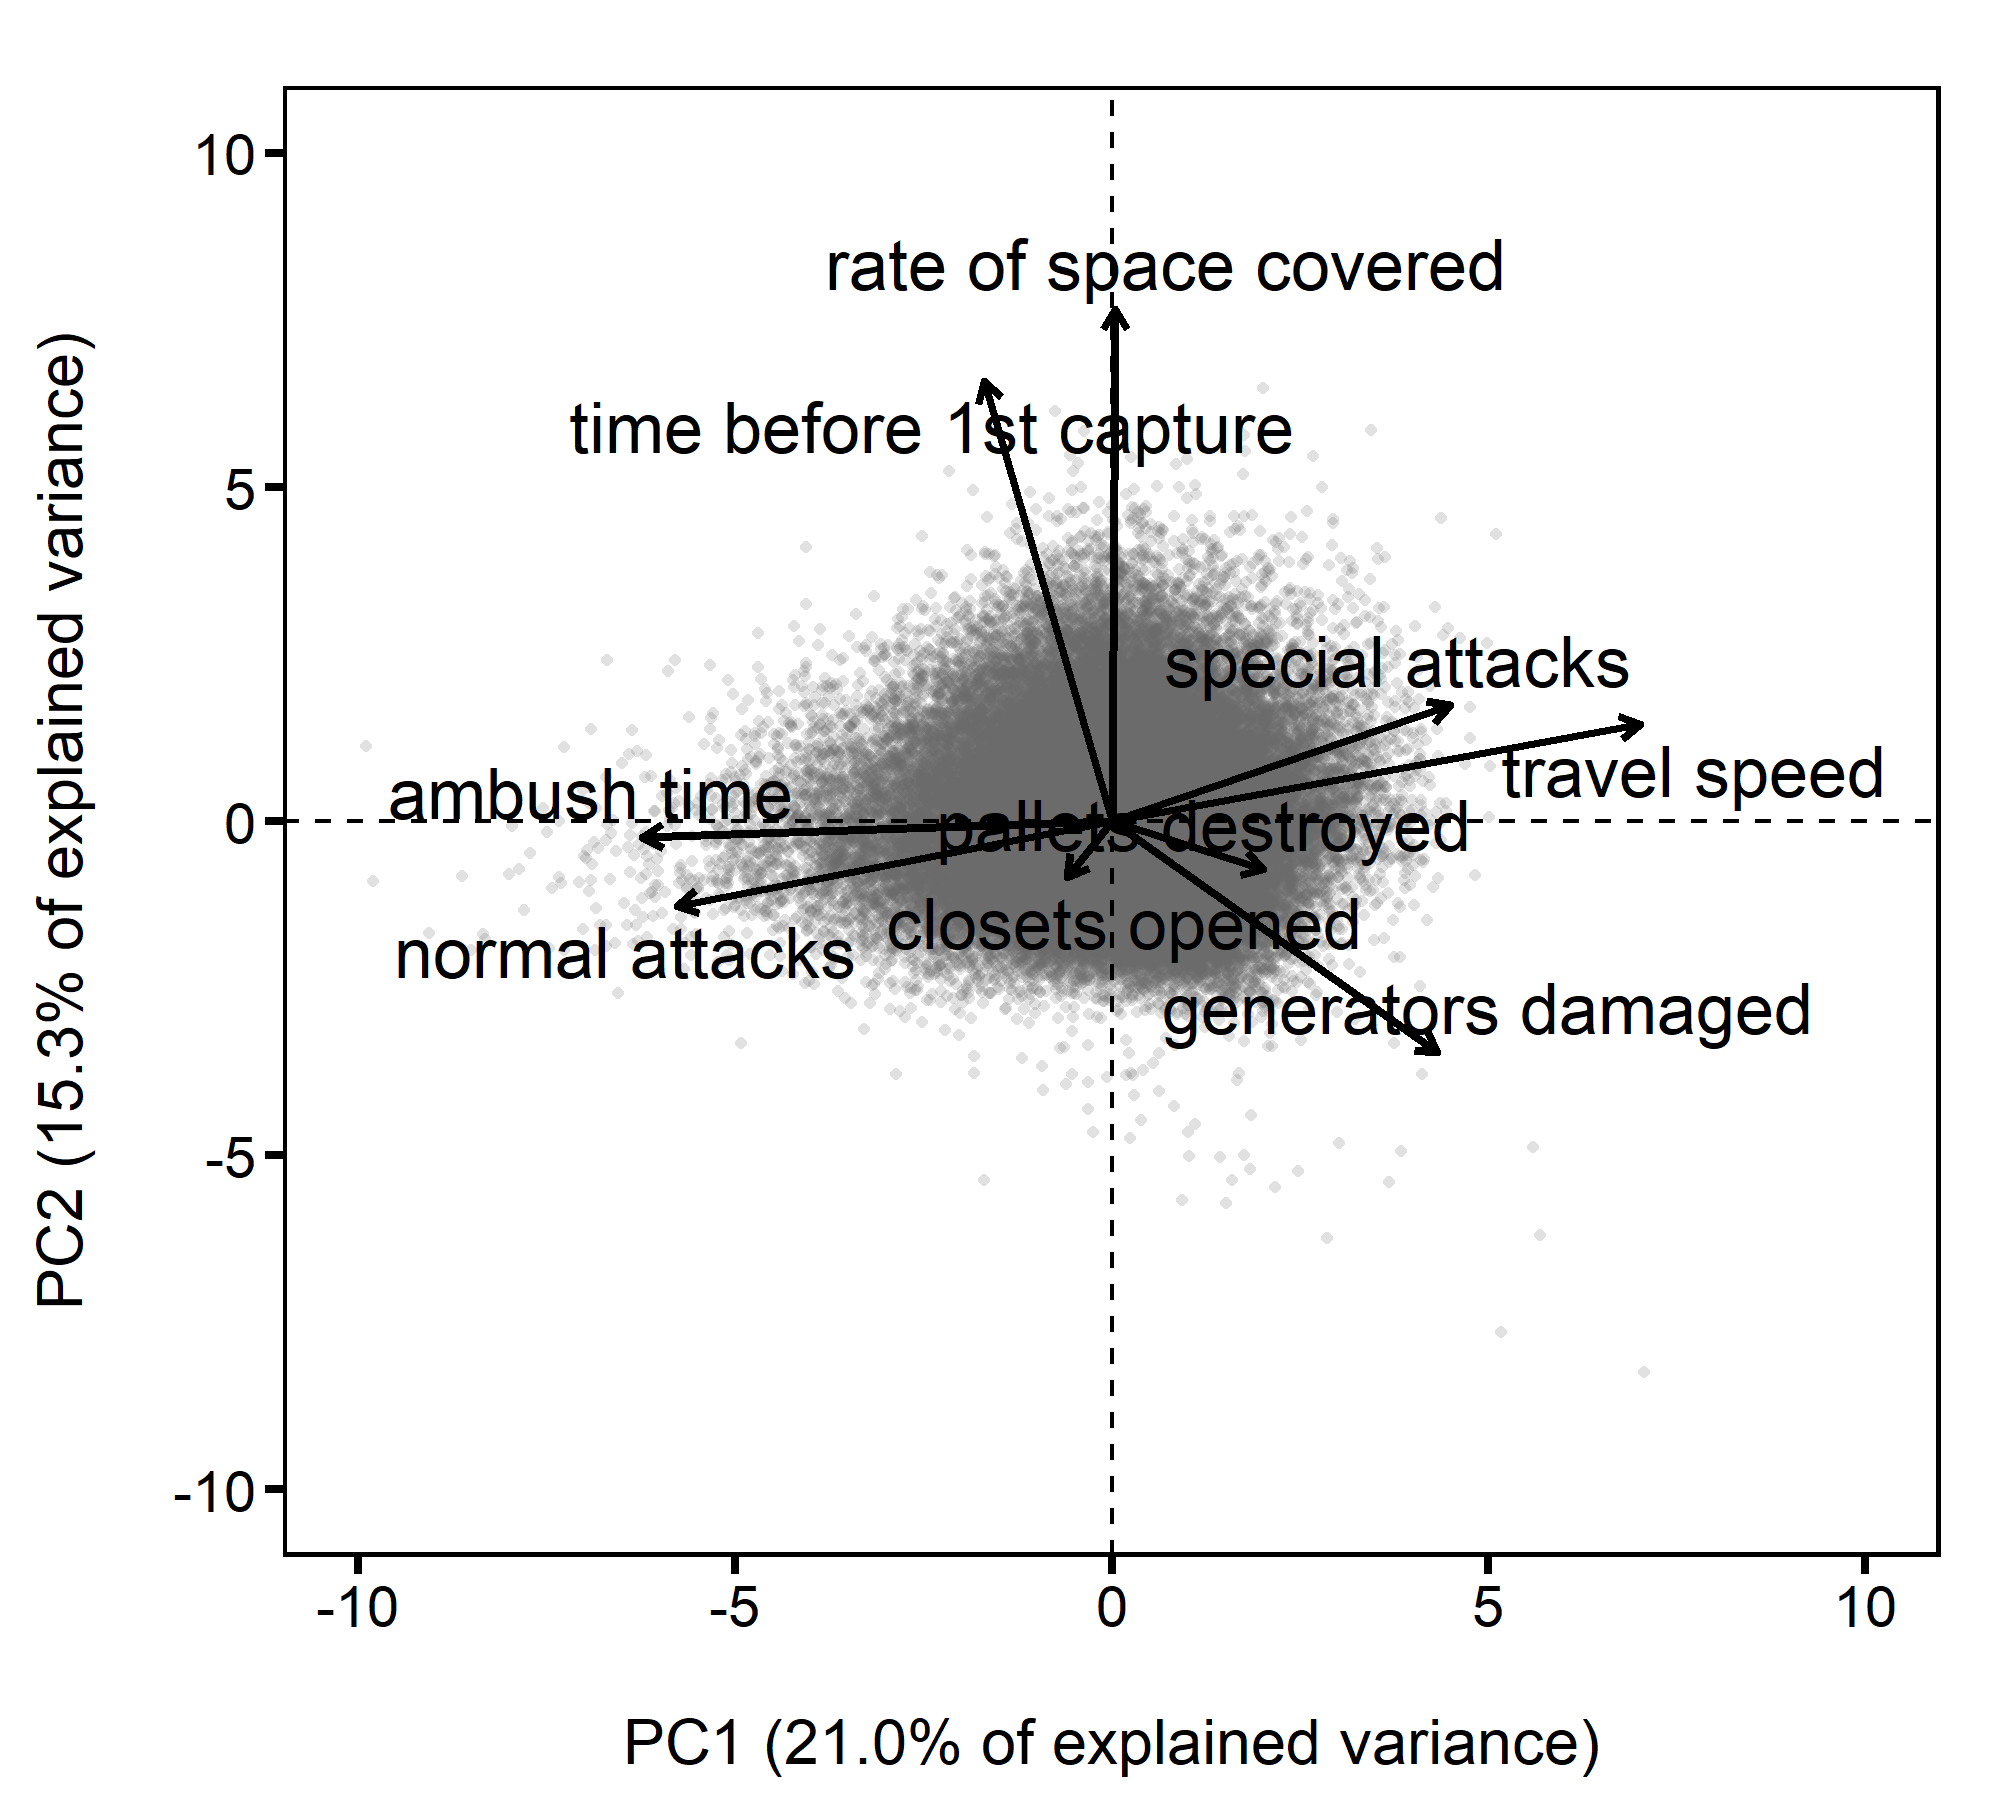
\includegraphics[width=0.8\linewidth]{C:/Users/maxim/OneDrive/Documents/GitHub/Chapter2/outputs/figures/suppmat_figures/02_figureS1}

\}

\textbackslash caption\{Biplot of the principal component analysis on
predator hunting behaviors. The variables presented in the main text
were selected based on their relative contribution (\%) to the first and
second principal components.\}\label{fig:Figure 1}
\textbackslash end\{figure\}

\newpage

\begin{figure}
\centering
\caption*{\textbf{Table S1:} Principal component loadings for all the predator behavioral traits.}
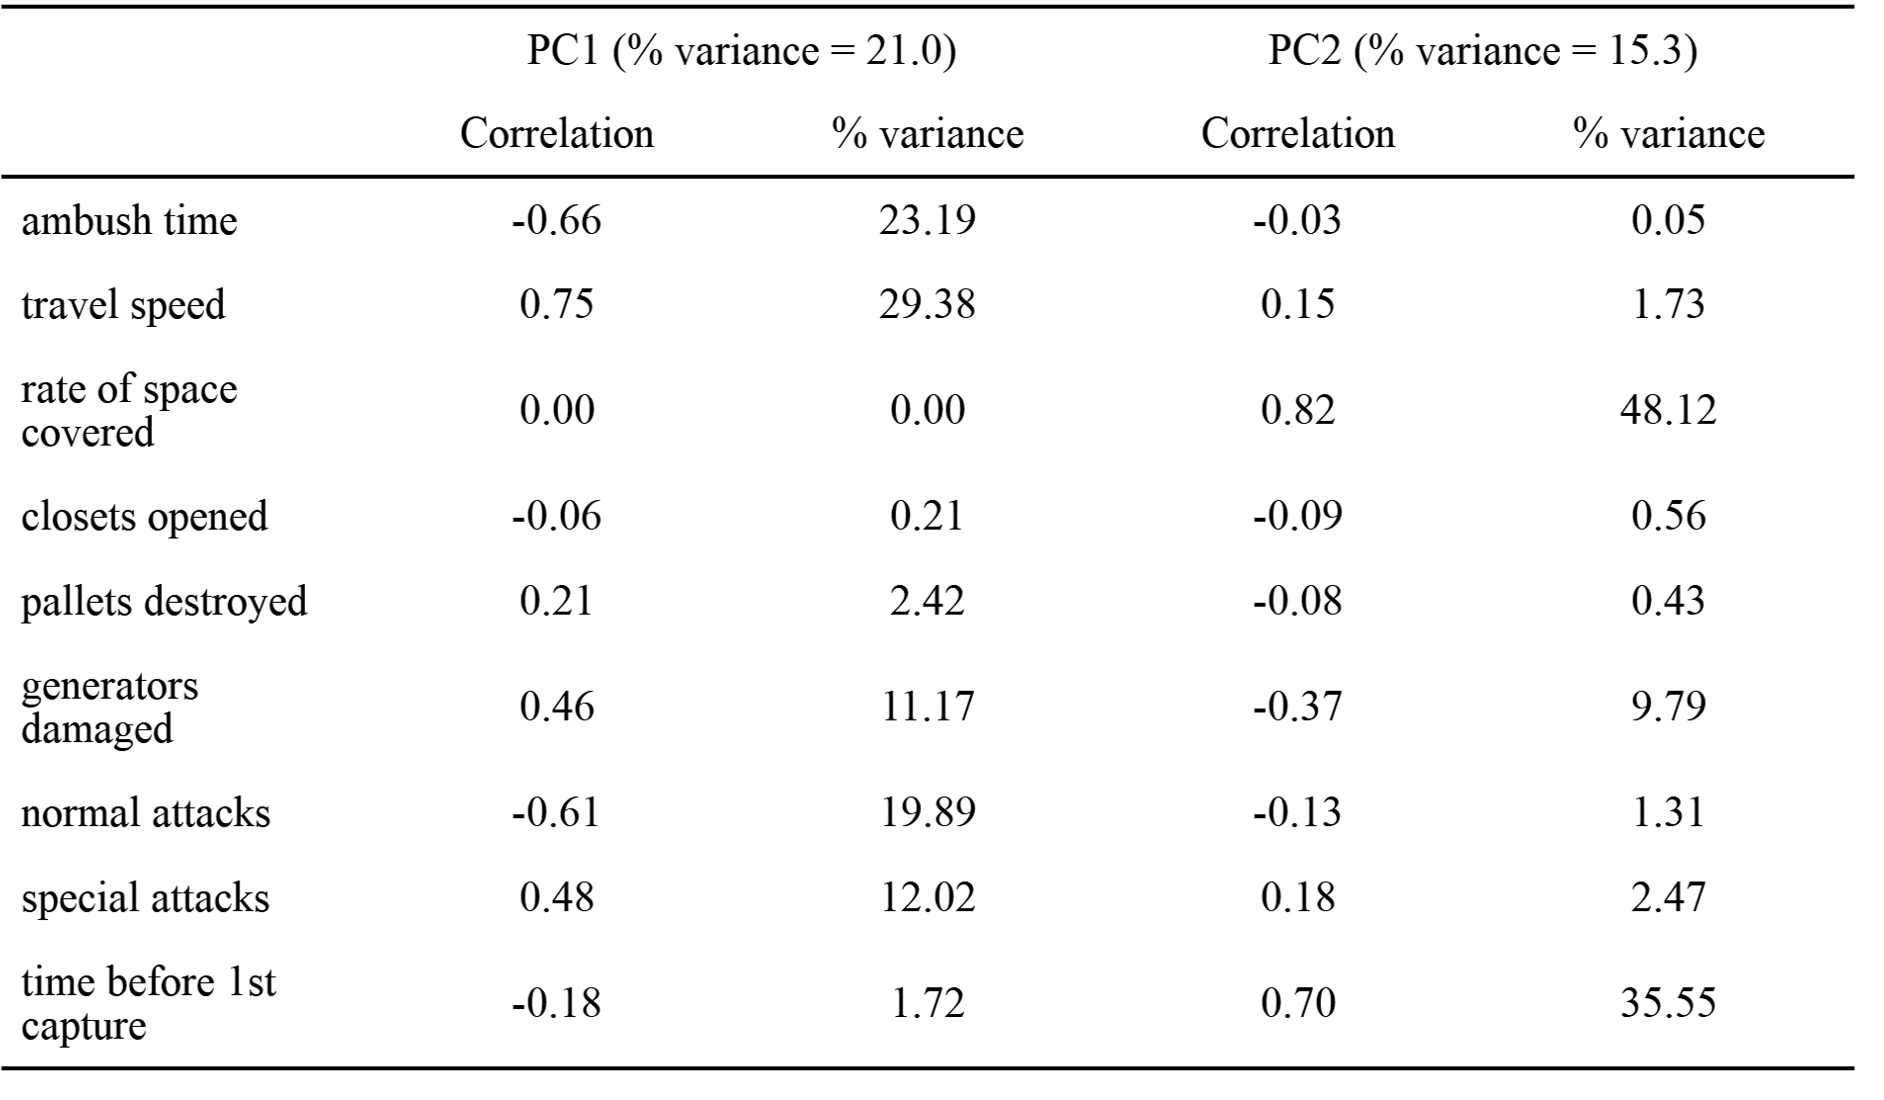
\includegraphics[width = \linewidth]{tableS1.png}
\end{figure}

\newpage

\begin{center}
\emph{Intra-class correlation coefficients of the predator behaviors for the three additional multivariate mixed-models}
\end{center}

After removing prey behavior as linear fixed effects (model 2), the
relative contribution (\%) of the game environments to the variation in
travel speed, the time spent guarding, and the time required to capture
the first prey was comparable to the first model (table S2). Thus, the
expression of these behaviors was similar among the game environments.
However, among environmental differences in the rate of space covered
increased (table S2). Results show that novice and experimented players
obtained similar ICCs for several of their random effects. However,
experimented players were more similar in their average behavior than
novice players.

\vspace{12pt}

\begin{figure}
\centering
\caption*{\textbf{Table S2:} Posterior means of the ICC estimates for the three additional multivariate mixed-models.}
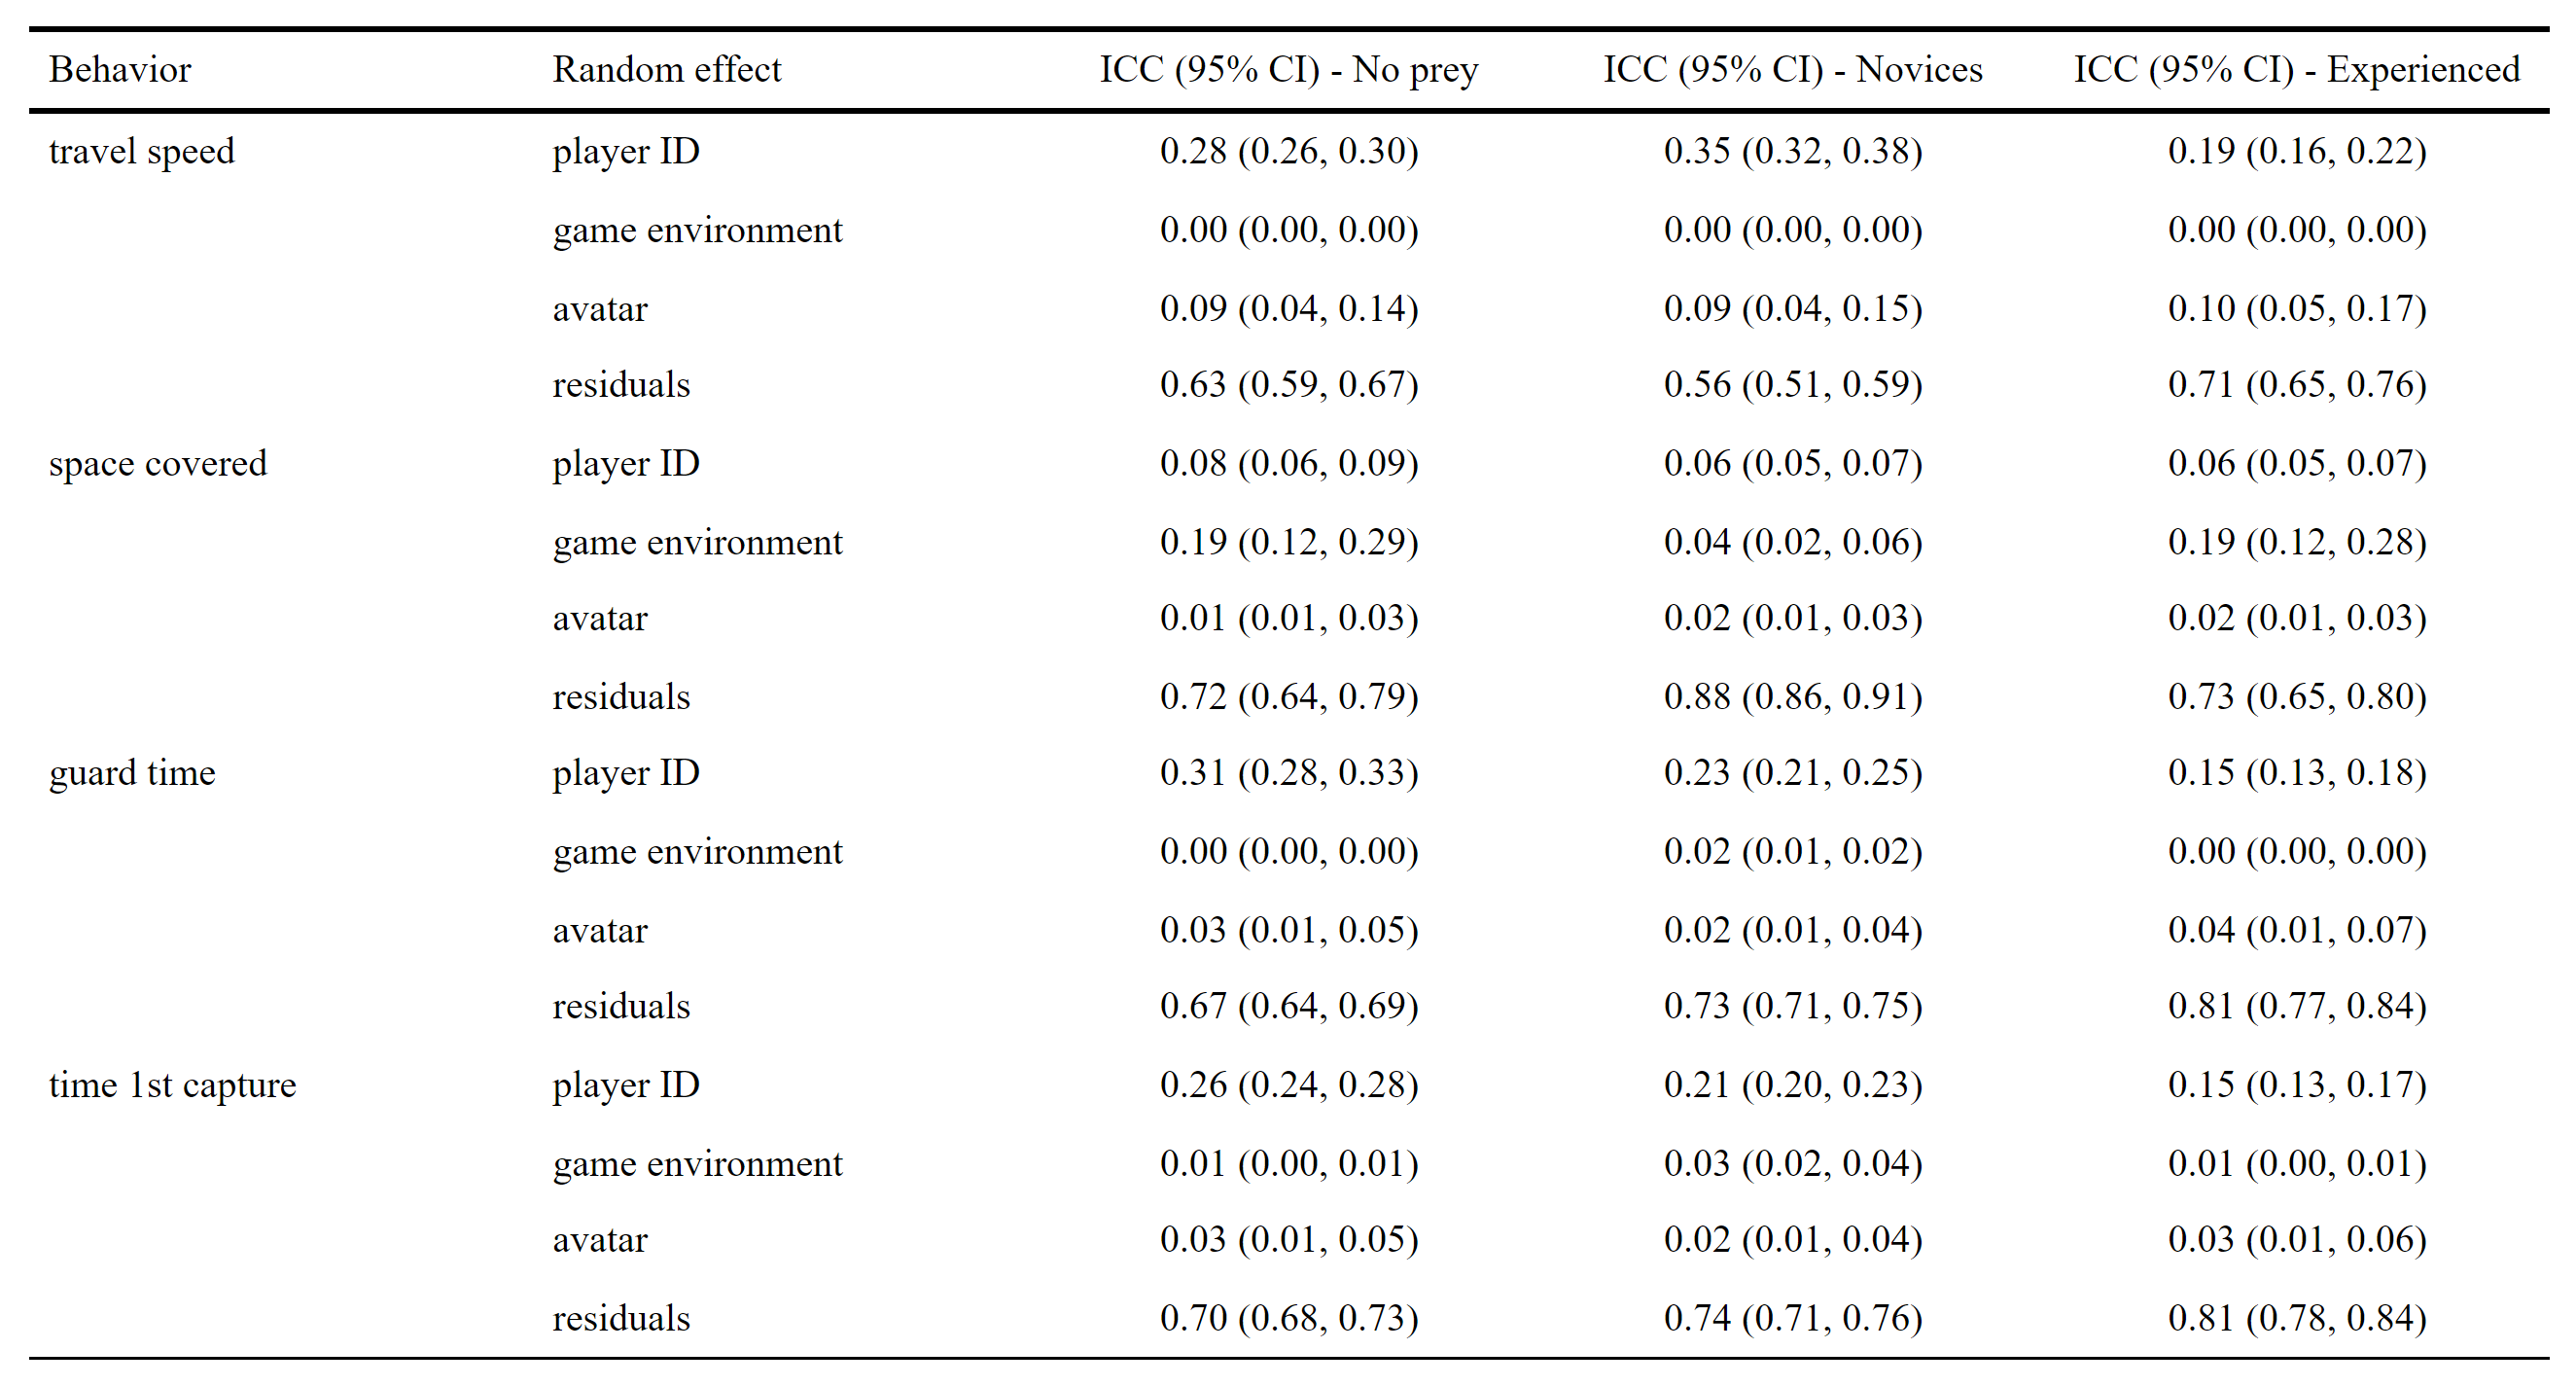
\includegraphics[width = \linewidth]{tableS2.png}
\end{figure}

\begin{figure}
\centering
\caption*{\textbf{Table S3:} Among-individual and within-individual behavioral correlations for the three additional multivariate mixed-models.}
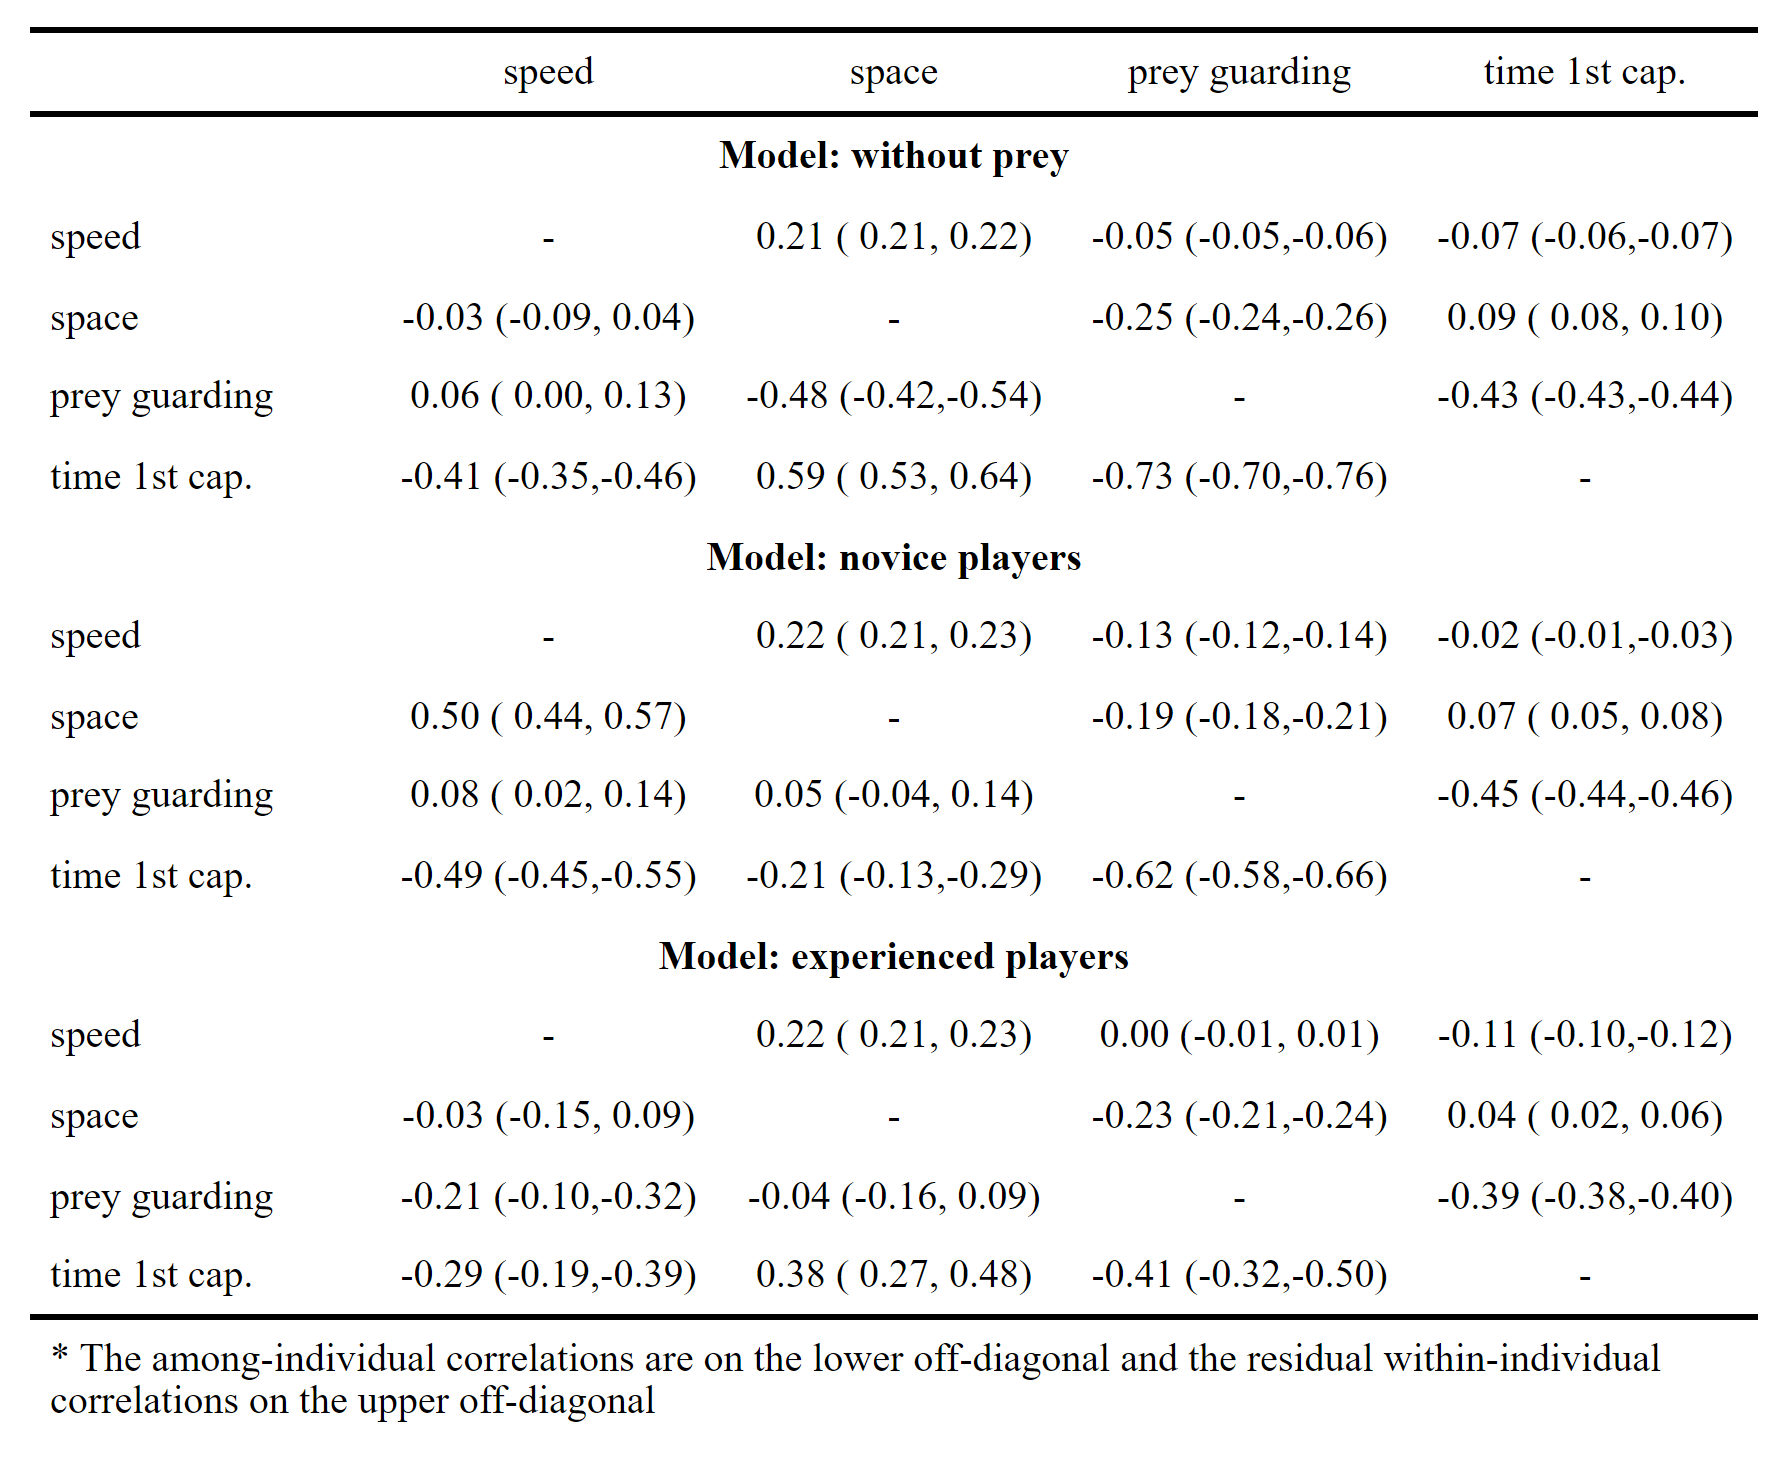
\includegraphics[width = \linewidth]{tableS3.png}
\end{figure}

\newpage

\begin{center}
\emph{Selection of the best hunting success model}
\end{center}

The model with the lowest expected log predictive density was chosen as
the best model for our interpretations of the relationship between
behavior and hunting success.

\begin{figure}
\centering
\caption*{\textbf{Table S4:} Summary table comparing the hunting success models based on approximate leave-one-out cross-validation}
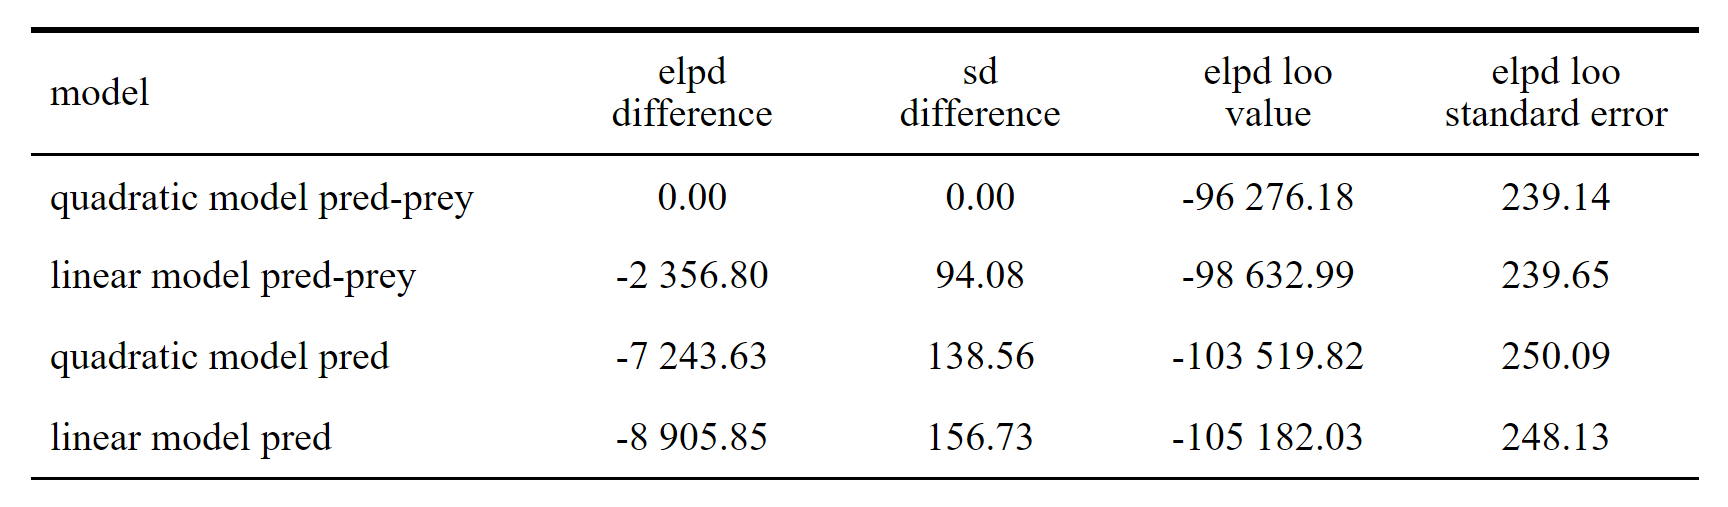
\includegraphics[width = \linewidth]{tableS4.png}
\end{figure}

\newpage

\begin{center}
\emph{Interactions between predator behavioral traits and hunting success}
\end{center}

Figure S2 shows the interacting effects of all the combinations of
predator behaviors on predator hunting success drawn from the parameters
presented on table 1 in the main text.

\begin{figure}
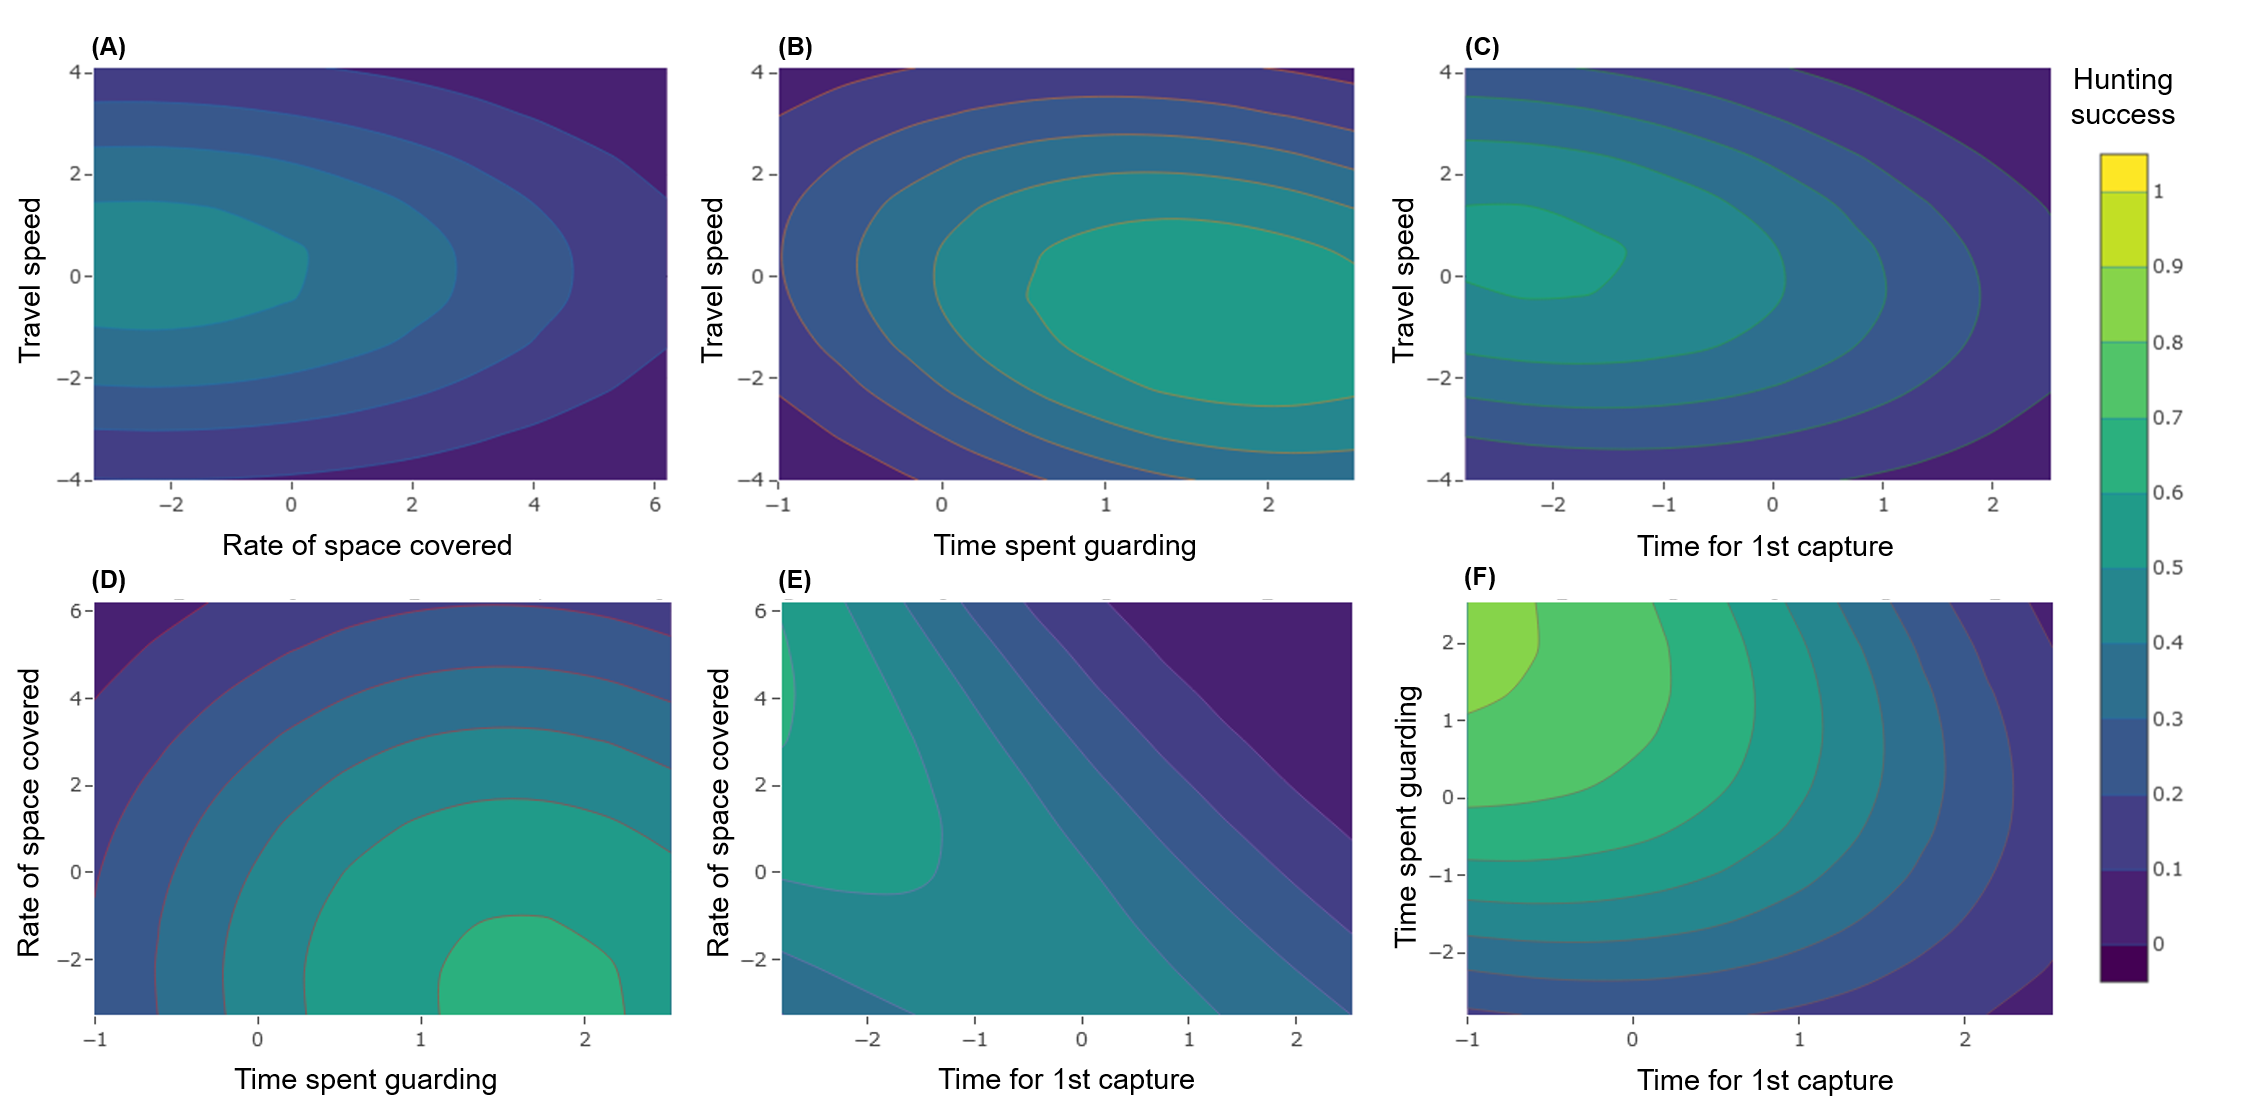
\includegraphics[width=1\linewidth]{C:/Users/maxim/OneDrive/Documents/GitHub/Chapter2/outputs/figures/suppmat_figures/04_figureS2} \caption{Interacting effects of the predator behaviors on hunting success. Hunting success is represented by the color gradient. We computed the plots by predicting the mean probability of capturing four prey based on the best quadratic approximation of the predator behavior interaction terms. (A) Travel speed and the rate of space covered. (B) Travel speed and the time spent guarding prey. (C) Time before the first capture and travel speed. (D) The rate of space covered and the time spent guarding. (E) The rate of space covered and the time before the first capture. (F) The time spent guarding prey and the time before the first capture.}\label{fig:Figure 2}
\end{figure}

\hypertarget{literature-cited}{%
\subsubsection{Literature Cited}\label{literature-cited}}

\hypertarget{refs}{}
\begin{cslreferences}
\leavevmode\hypertarget{ref-Kassambara.Mundt2020}{}%
Kassambara A, Mundt F. 2020 Apr 1. Factoextra: Extract and Visualize the
Results of Multivariate Data Analyses.

\leavevmode\hypertarget{ref-Le.etal2008}{}%
Lê S, Josse J, Husson F. 2008. FactoMineR: An R Package for Multivariate
Analysis. J Stat Softw. 25(1, 1):1--18.

\leavevmode\hypertarget{ref-nakagawaCoefficientDeterminationR22017}{}%
Nakagawa S, Johnson PCD, Schielzeth H. 2017. The coefficient of
determination R2 and intra-class correlation coefficient from
generalized linear mixed-effects models revisited and expanded. J R Soc
Interface. 14(134):20170213.
\end{cslreferences}

\end{document}
